\documentclass{standalone}
\usepackage{tikz}
\usetikzlibrary{patterns, positioning}


\begin{document}
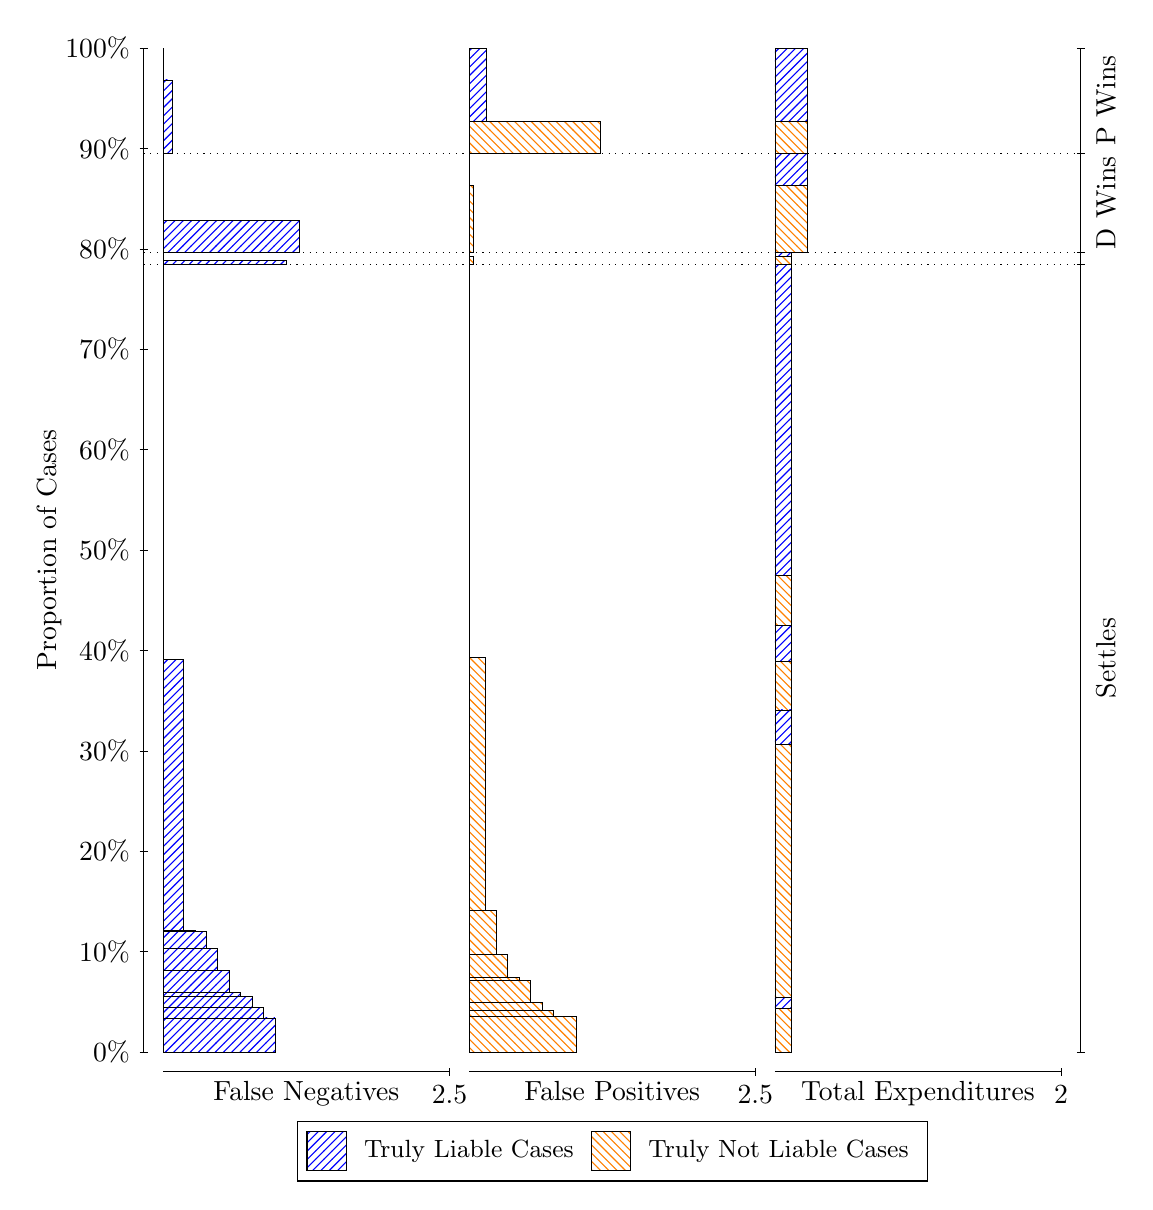
\begin{tikzpicture}
\draw[black, very thin] (1.5,1.75) -- (1.5,14.5);
\node[rotate=90, text=black, anchor=center] at (0.3, 8.125) {Proportion of Cases};
\draw[black, very thin] (1.45,1.75) -- (1.55,1.75);
\node[text=black, anchor=east] at (1.45, 1.75) {0\%};
\draw[black, very thin] (1.45,3.025) -- (1.55,3.025);
\node[text=black, anchor=east] at (1.45, 3.025) {10\%};
\draw[black, very thin] (1.45,4.3) -- (1.55,4.3);
\node[text=black, anchor=east] at (1.45, 4.3) {20\%};
\draw[black, very thin] (1.45,5.575) -- (1.55,5.575);
\node[text=black, anchor=east] at (1.45, 5.575) {30\%};
\draw[black, very thin] (1.45,6.85) -- (1.55,6.85);
\node[text=black, anchor=east] at (1.45, 6.85) {40\%};
\draw[black, very thin] (1.45,8.125) -- (1.55,8.125);
\node[text=black, anchor=east] at (1.45, 8.125) {50\%};
\draw[black, very thin] (1.45,9.4) -- (1.55,9.4);
\node[text=black, anchor=east] at (1.45, 9.4) {60\%};
\draw[black, very thin] (1.45,10.675) -- (1.55,10.675);
\node[text=black, anchor=east] at (1.45, 10.675) {70\%};
\draw[black, very thin] (1.45,11.95) -- (1.55,11.95);
\node[text=black, anchor=east] at (1.45, 11.95) {80\%};
\draw[black, very thin] (1.45,13.225) -- (1.55,13.225);
\node[text=black, anchor=east] at (1.45, 13.225) {90\%};
\draw[black, very thin] (1.45,14.5) -- (1.55,14.5);
\node[text=black, anchor=east] at (1.45, 14.5) {100\%};

\draw[black, very thin] (13.4,1.75) -- (13.4,14.5);
\draw[black, very thin] (13.35,1.75) -- (13.45,1.75);
\node[anchor=west] at (13.35, 1.75) {};
\draw[black, very thin] (13.35,11.756) -- (13.45,11.756);
\node[anchor=west] at (13.35, 11.756) {};
\draw[black, very thin] (13.35,11.902) -- (13.45,11.902);
\node[anchor=west] at (13.35, 11.902) {};
\draw[black, very thin] (13.35,13.163) -- (13.45,13.163);
\node[anchor=west] at (13.35, 13.163) {};
\draw[black, very thin] (13.35,14.5) -- (13.45,14.5);
\node[anchor=west] at (13.35, 14.5) {};

\draw[black, very thin, pattern color=blue, pattern=north east lines] (1.75,1.75) rectangle (3.167,2.1827);
\draw[black, very thin, pattern color=blue, pattern=north east lines] (1.75,2.1827) rectangle (3.0217,2.3202);
\draw[black, very thin, pattern color=blue, pattern=north east lines] (1.75,2.3202) rectangle (2.8763,2.46);
\draw[black, very thin, pattern color=blue, pattern=north east lines] (1.75,2.46) rectangle (2.731,2.5019);
\draw[black, very thin, pattern color=blue, pattern=north east lines] (1.75,2.5019) rectangle (2.5857,2.7857);
\draw[black, very thin, pattern color=blue, pattern=north east lines] (1.75,2.7857) rectangle (2.4403,3.07);
\draw[black, very thin, pattern color=blue, pattern=north east lines] (1.75,3.07) rectangle (2.295,3.285);
\draw[black, very thin, pattern color=blue, pattern=north east lines] (1.75,3.285) rectangle (2.1497,3.2964);
\draw[black, very thin, pattern color=blue, pattern=north east lines] (1.75,3.2964) rectangle (2.0043,6.7394);
\draw[black, very thin, pattern color=orange, pattern=north west lines] (1.75,6.7394) rectangle (1.75,11.756);
\draw[black, very thin, pattern color=blue, pattern=north east lines] (1.75,11.756) rectangle (3.3123,11.804);
\draw[black, very thin, pattern color=orange, pattern=north west lines] (1.75,11.804) rectangle (1.75,11.902);
\draw[black, very thin, pattern color=blue, pattern=north east lines] (1.75,11.902) rectangle (3.4758,12.307);
\draw[black, very thin, pattern color=orange, pattern=north west lines] (1.75,12.307) rectangle (1.75,13.163);
\draw[black, very thin, pattern color=blue, pattern=north east lines] (1.75,13.163) rectangle (1.859,14.095);
\draw[black, very thin, pattern color=orange, pattern=north west lines] (1.75,14.095) rectangle (1.75,14.5);
\draw[black, very thin, pattern color=orange, pattern=north west lines] (5.6333,1.75) rectangle (6.9958,2.2016);
\draw[black, very thin, pattern color=orange, pattern=north west lines] (5.6333,2.2016) rectangle (6.8505,2.2056);
\draw[black, very thin, pattern color=orange, pattern=north west lines] (5.6333,2.2056) rectangle (6.7052,2.281);
\draw[black, very thin, pattern color=orange, pattern=north west lines] (5.6333,2.281) rectangle (6.5598,2.3807);
\draw[black, very thin, pattern color=orange, pattern=north west lines] (5.6333,2.3807) rectangle (6.4145,2.6561);
\draw[black, very thin, pattern color=orange, pattern=north west lines] (5.6333,2.6561) rectangle (6.2692,2.698);
\draw[black, very thin, pattern color=orange, pattern=north west lines] (5.6333,2.698) rectangle (6.1238,2.9931);
\draw[black, very thin, pattern color=orange, pattern=north west lines] (5.6333,2.9931) rectangle (5.9785,3.5485);
\draw[black, very thin, pattern color=orange, pattern=north west lines] (5.6333,3.5485) rectangle (5.8332,6.7661);
\draw[black, very thin, pattern color=blue, pattern=north east lines] (5.6333,6.7661) rectangle (5.6333,11.756);
\draw[black, very thin, pattern color=orange, pattern=north west lines] (5.6333,11.756) rectangle (5.6878,11.854);
\draw[black, very thin, pattern color=blue, pattern=north east lines] (5.6333,11.854) rectangle (5.6333,11.902);
\draw[black, very thin, pattern color=orange, pattern=north west lines] (5.6333,11.902) rectangle (5.6878,12.758);
\draw[black, very thin, pattern color=blue, pattern=north east lines] (5.6333,12.758) rectangle (5.6333,13.163);
\draw[black, very thin, pattern color=orange, pattern=north west lines] (5.6333,13.163) rectangle (7.3047,13.568);
\draw[black, very thin, pattern color=blue, pattern=north east lines] (5.6333,13.568) rectangle (5.8513,14.5);
\draw[black, very thin, pattern color=orange, pattern=north west lines] (9.5167,1.75) rectangle (9.721,2.3054);
\draw[black, very thin, pattern color=blue, pattern=north east lines] (9.5167,2.3054) rectangle (9.721,2.443);
\draw[black, very thin, pattern color=orange, pattern=north west lines] (9.5167,2.443) rectangle (9.721,5.6606);
\draw[black, very thin, pattern color=blue, pattern=north east lines] (9.5167,5.6606) rectangle (9.721,6.0933);
\draw[black, very thin, pattern color=orange, pattern=north west lines] (9.5167,6.0933) rectangle (9.721,6.7056);
\draw[black, very thin, pattern color=blue, pattern=north east lines] (9.5167,6.7056) rectangle (9.721,7.1711);
\draw[black, very thin, pattern color=orange, pattern=north west lines] (9.5167,7.1711) rectangle (9.721,7.8018);
\draw[black, very thin, pattern color=blue, pattern=north east lines] (9.5167,7.8018) rectangle (9.721,11.756);
\draw[black, very thin, pattern color=orange, pattern=north west lines] (9.5167,11.756) rectangle (9.721,11.854);
\draw[black, very thin, pattern color=blue, pattern=north east lines] (9.5167,11.854) rectangle (9.721,11.902);
\draw[black, very thin, pattern color=orange, pattern=north west lines] (9.5167,11.902) rectangle (9.9254,12.758);
\draw[black, very thin, pattern color=blue, pattern=north east lines] (9.5167,12.758) rectangle (9.9254,13.163);
\draw[black, very thin, pattern color=orange, pattern=north west lines] (9.5167,13.163) rectangle (9.9254,13.568);
\draw[black, very thin, pattern color=blue, pattern=north east lines] (9.5167,13.568) rectangle (9.9254,14.5);
\draw[black, dotted] (1.5,11.756) -- (13.4,11.756);
\draw[black, dotted] (1.5,11.902) -- (13.4,11.902);
\draw[black, dotted] (1.5,13.163) -- (13.4,13.163);
\draw[black, very thin] (1.75,1.5) -- (5.3833,1.5);
\node[text=black, anchor=north] at (3.5667, 1.5) {False Negatives};
\draw[black, very thin] (5.3833,1.45) -- (5.3833,1.55);
\node[text=black, anchor=north] at (5.3833, 1.45) {2.5};

\draw[black, very thin] (5.6333,1.5) -- (9.2667,1.5);
\node[text=black, anchor=north] at (7.45, 1.5) {False Positives};
\draw[black, very thin] (9.2667,1.45) -- (9.2667,1.55);
\node[text=black, anchor=north] at (9.2667, 1.45) {2.5};

\draw[black, very thin] (9.5167,1.5) -- (13.15,1.5);
\node[text=black, anchor=north] at (11.333, 1.5) {Total Expenditures};
\draw[black, very thin] (13.15,1.45) -- (13.15,1.55);
\node[text=black, anchor=north] at (13.15, 1.45) {2};

\node[text=black, centered, rotate=90] at (13.72, 6.7528) {Settles};

\node[text=black, centered, rotate=90] at (13.72, 12.533) {D Wins};
\node[text=black, centered, rotate=90] at (13.72, 13.832) {P Wins};

\draw (7.449999999999999,1.5) node[draw=none] (baseCoordinate) {};
\begin{scope}[align=center]
        \matrix[scale=0.5, draw=black, below=0.5cm of baseCoordinate, nodes={draw}, column sep=0.1cm]{
            \node[rectangle, draw, minimum width=0.5cm, minimum height=0.5cm, pattern color=blue, pattern=north east lines] {}; &
            \node[draw=none, font=\small, text=black] (B) {Truly Liable Cases}; &
            \node[rectangle, draw, minimum width=0.5cm, minimum height=0.5cm, pattern color=orange, pattern=north west lines] {}; &
            \node[draw=none, font=\small, text=black] (B) {Truly Not Liable Cases}; \\
            };
\end{scope}

\end{tikzpicture}
\end{document}